\documentclass[11pt, a4paper, spanish]{article}

%%%%%%%%%% COMIENZO DEL PREAMBULO %%%%%%%%%%

%Info sobre este documento
\author{Martin Cammi}
\title{Trabajo Pr'actico de Ingenier'ia del software I}

%\usepackage{infostyle}                                                  % provee un look & feel similar a un documento Word
\usepackage[top=2.5cm, bottom=2.5cm, left=2.5cm, right=2.5cm]{geometry}  % m\'argenes
\usepackage[ansinew]{inputenc}                                           % permite que los acentos del estilo \'a\'e\'i\'o\'u salgan joya
\usepackage[spanish, activeacute]{babel}                                 % idioma espa\~{n}ol, acentos f\'aciles y deletreo de palabras
\usepackage{indentfirst}                                                 % permite indentar un parrafo a mano
\usepackage{caratula}                                                    % incluye caratula est\'andar
\usepackage{graphicx}                                                    % permite insertar gr\'aficos
\usepackage{color}                                                       % permite el uso de colores en el documento
\usepackage[pdfcreator={TexLive!, LaTeX2e con TeXnicCenter;-)},
			pdfauthor={Grupo 2"},
			pdftitle={Base de Datos - Trabajo practico:},
			pdfsubject={Trabajo Practico de Buffer Manager},
			pdfkeywords={MER, MR},
			pdfstartview=FitH,            % Fits the width of the page to the window
			bookmarksnumbered,            % los bookmarks numerados se ven mejor...
			colorlinks,                   % links con bellos colores
			linkcolor=magenta]            % permite cambiar el color de los links
			{hyperref}                    % Permite jugar con algunas cosas que aparecer\'an en el PDF final
\usepackage{hyperref}
\usepackage{rotating}
\usepackage{ulem}
\usepackage[dash]{dashundergaps}


%\selectlanguage{spanish}

\linespread{1.3}                    % interlineado equivalente al 1.5 l\'ineas de Word...
\pagestyle{myheadings}              %encabezado personalizable con \markboth{}{}
\markboth{}{Trabajo pr\'actico 2 (Cammi, De Sousa) }
\headsep = 30pt                     % separaci\'on entre encabezado y comienzo del p\'arrafo

%\addtolength{\oddsidemargin}{-2cm}	% configuracion IDEAL!!!
%\addtolength{\textwidth}{4cm}
%\addtolength{\textheight}{2cm}

% macro 'todo' para To-Do's
\def\todo#1{\textcolor{red}{#1}}

% Macro 'borde' para un texto con borde
\newsavebox{\fmbox}
\newenvironment{borde}[1]
{\begin{lrbox}{\fmbox}\begin{minipage}{#1}}
{\end{minipage}\end{lrbox}\fbox{\usebox{\fmbox}}\\[10pt]}

%%%%%%%%%% FIN DEL PREAMBULO %%%%%%%%%%

\begin{document}

\materia{Base de Datos}
\submateria{Segundo Cuatrimestre de 2012}
\titulo{Trabajo pr\'actico 2}
\subtitulo{Buffer Manager y estrategias de reemplazo de p'aginas}
\grupo{Grupo 2}

\integrante{Cammi, Mart\'in}{676/02}{martincammi@gmail.com}
\integrante{De Sousa, Mariano}{389/08}{marian\_sabianaa@hotmail.com}

\maketitle

\thispagestyle{empty}

\tableofcontents

\newpage

% Conviene poner las secciones como diferentes archivos,
% sobre todo cuando se trabaja en equipo.
% Es m\'as f\'acil para sincronizar mediante control de versiones.
%\input{Introducci\'on}


% BEGIN Ejemplos de uso

	%\section{Una secci\'on}
	%\label{sec:unaSeccion}
	%Hola! Soy una Secci\'on
	%	\subsection{Una subsecci\'on}
	%		Y yo soy una subsecci\'on!!!
	%		\subsubsection{Una subsubsecci\'on}
	%			Y yo soy una sub-subsecci\'on!!!
	%			\paragraph{Un p\'arrafo\\}
	%				Y yo soy un p\'arrafo, porque no hay mas sub-sub-sub-subsecciones!!!

	%\section{Otra secci\'on}
	%	Como pudimos ver en la secci\'on \ref{sec:unaSeccion}, esto es una demo de una referencia a una secci\'on.
	
	%	Tambi\'en podemos hacer referencia a la p\'agina de la secci\'on:\\[10pt]
	
		% Ejemplo de uso de un borde (falta pulir para que no tire un warning!)
	%	\begin{borde}{0.98\textwidth}
	%		En la p\'agina \pageref{sec:unaSeccion}, hay una secci\'on pilla...
	%	\end{borde}

% END Ejemplos de uso

\newpage 
\section{Investigaci'on sobre estrategia de reemplazo de p'aginas de Oracle}

\subsection{Introducci\'on}

===Hacer referencia bien a la caché indicando que es y el termino caché del buffer de que buffer\\

A lo largo de este trabajo analizaremos el algoritmo de \textit{Touch Count} dise\~{n}ado por \textit{Oracle} para administrar en memoria las p\'aginas que se
traen de la base de datos con el objetivo de evitar los accesos a disco utilizando dicha memoria de a manera m\'as eficiente.\\

Inicialmente Oracle utilizaba para el algoritmo de manejo de \textit{cach\'e} lo que se conoce como algoritmo LRU (Least Recently Used). Este algoritmo, 
descripto m\'as adelante se basa en priorizar en la cach\'e las p\'aginas de disco más referenciadas descartando las menos usadas recientemente 
(definici\'on de LRU).

Un caso muy com\'un que presenta un problema a este algoritmo son los full scan, los cuales recorren todos los registros de una tabla coloc\'andolos en 
la \textit{cach'e} y pisando todo historial previo. As\'i por ejemplo, si la cache del buffer tiene 300 bloques y un escaneo completo de una 
tabla est'a recibiendo 400 bloques en la cache del buffer, todos los bloques populares desaparecer'an. \\

Para superar este problema, Oracle propuso un algoritmo modificado de LRU al que denomin\'o \textit{Touch Count}
  
\subsection{Algoritmo \textit{Touch Count}}

El algoritmo \textit{Touch Count} utiliza el mismo esp\'iritu que sus predecesores LRU y MRU, solo que en una mezcla de ambos. Por un lado priorizar\'a
mantener en la cach\'e las p\'aginas m\'as referenciadas y descartar las menos pero a su modo, cualquier p\'agina que ingrese deber\'a competir 
con otras existentes en la cach\'e por permanecer en la misma, para ello el algoritmo llevará un conteo de cuantas veces fue referenciada. Este n\'umero
de referencias a la p\'agina se denomina \textit{Touch Count}.

\subsection{Problem\'atica que resuelve}

Uno de los problemas que el \textit{Touch Count} resuelve es el de las r\'afagas de acceso a p\'aginas. En un full scan por ejemplo m\'ultiples p\'aginas
son referenciadas y en algoritmos como 

\subsection{Ventajas y desventajas}

\newpage 
\section{Implementaci'on estrategias de reemplazo de p'aginas}

\subsection{Algoritmo de LRU}

El algoritmo LRU (Least Recently Used) funciona de la siguiente manera, intentando mantener en memoria las p\'aginas m\'as recientemente usadas
y en caso de necesitar remover alguna elegir de entre alguna de las menos recientemente usadas.\\

El siguiente es un ejemplo de como las cach\'e se va actualizando mediante el algoritmo LRU.

El siguiente gr\'afico se lee de izquierda a derecha de arriba abajo. La primera hilera de n\'umeros corresponde a la traza de p\'aginas que intentan ser 
accedidas. Debajo de ella aparece en forma vertical la cach\'e y como se va llenando a medida que c\'ada p\'agina de la traza es referenciada.\\ 

Marcaremos con amarillo cuando ocurra un \textit{Hit} y con gris cuando ocurra un \textit{Miss}.
Cuando una p\'agina sea referenciada la marcaremos en la cach\'e en negrita para saber que fue la m\'as recientemente accedida.\\

\begin{center}
		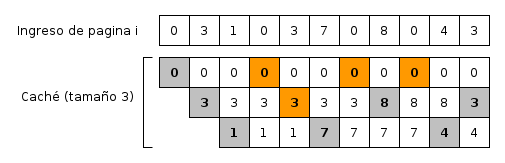
\includegraphics[scale=0.65]{diagramas/LRUAlgorithm.png}\\
\end{center}

As\'i en el ejemplo, 
\begin{itemize}
	\item{ Se referencia inicialmente la p\'agina 0, como la cach\'e se encuentra vac\'ia se produce un \textit{Miss}, y se prodece a agregar
		la p\'agina 0 a la cach\'e.}
	\item{ Se referencia a la p\'agina 3, como no existe en la cach\'e (ya que solo posee la p\'agina 0 agregada anterioremente) se produce 
		un \textit{Miss} y se prodece a agregar la p\'agina 3 a la cach\'e.}
	\item{ Se referencia a la p\'agina 1, como no existe en la cach\'e se produce un \textit{Miss} y se prodece a agregar la p\'agina 1 a la cach\'e.}
	\item{ Se referencia a la p\'agina 0, como existe en la cach\'e se produce un \textit{Hit}. }
	\item{ Se referencia a la p\'agina 3, como existe en la cach\'e se produce un \textit{Hit}. }
	\item{ Se referencia a la p\'agina 7, como no existe en la cach\'e se produce un \textit{Miss} y se prodece a agregar la p\'agina 7 a la cach\'e
		reemplazando la menos recientemente usada que es la p\'agina 1. }
	\item{ Se referencia a la p\'agina 0, como existe en la cach\'e se produce un \textit{Hit}. }
	\item{ Se referencia a la p\'agina 8, como no existe en la cach\'e se produce un \textit{Miss} y se prodece a agregar la p\'agina 8 a la cach\'e
		reemplazando la menos recientemente usada que es la p\'agina 3. }
	\item{ Se referencia a la p\'agina 0, como existe en la cach\'e se produce un \textit{Hit}. }
	\item{ Se referencia a la p\'agina 4, como no existe en la cach\'e se produce un \textit{Miss} y se prodece a agregar la p\'agina 4 a la cach\'e
		reemplazando la menos recientemente usada que es la p\'agina 7. }
	\item{ Se referencia a la p\'agina 3, como no existe en la cach\'e (porque ya fue desalojada) se produce un \textit{Miss} y se prodece a agregar 
		la p\'agina 3 a la cach\'e reemplazando la menos recientemente usada que es la p\'agina 8. }
\end{itemize}

Es interesante notar que una p\'agina no ser\'a desalojada hasta tanto se hayan referenciado al menos una vez a todas las otras, ya que de esta forma
la p\'agina inicial se convertiría en la menos recientemente usada.\\

\noindent{\emph{Cantidad de Hits:} 4} \\
\emph{Cantidad de Miss:} 7, con un total de 3 \emph{Miss} iniciales y 4 \emph{Miss} a lo largo de la traza.\\
\emph{Predicci\'on:} Este enfoque intenta predecir que p\'aginas que fueron referenciadas posiblemente lo sean en un per\'iodo corto de tiempo.\\
\emph{Desventajas:} Una desventaja es que un full scan sobre una tabla barrer\'a por completo con todas las entradas de la cach\'e.\\
\emph{Ventajas:} \\

\newpage
\subsection{Algoritmo de MRU}

El algoritmo MRU (Most Recently Used) funciona a la inversa de \textit{LRU}, intentando mantener en memoria las p\'aginas menos recientemente usadas
y en caso de necesitar remover alguna elegir de entre alguna de las m\'as recientemente usadas.

El siguiente es un ejemplo de como las cach\'e se va actualizando mediante el algoritmo LRU.

\begin{center}
		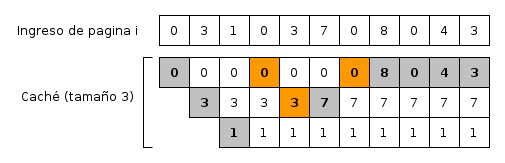
\includegraphics[scale=0.65]{diagramas/MRUAlgorithm.png}\\
\end{center}

El gr\'afico anterior se lee de izquierda a derecha de arriba abajo. La primera hilera de n\'umeros corresponde a la traza de p\'aginas que intentan ser 
accedidas. Debajo de ella aparece en forma vertical la cach\'e y como se va llenando a medida que c\'ada p\'agina de la traza es referenciada.\\ 

Marcaremos con amarillo cuando ocurra un \textit{Hit} y con gris cuando ocurra un \textit{Miss}.
Cuando una p\'agina sea referenciada la marcaremos en la cach\'e en negrita para saber que fue la m\'as recientemente accedida.\\

As\'i en el ejemplo, 

\begin{itemize}
	\item{ Se referencia inicialmente la p\'agina 0, como la cach\'e se encuentra vac\'ia se produce un \textit{Miss}, y se prodece a agregar
		la p\'agina 0 a la cach\'e.}
	\item{ Se referencia a la p\'agina 3, como no existe en la cach\'e (ya que solo posee la p\'agina 0 agregada anterioremente) se produce 
		un \textit{Miss} y se prodece a agregar la p\'agina 3 a la cach\'e.}
	\item{ Se referencia a la p\'agina 1, como no existe en la cach\'e se produce un \textit{Miss} y se prodece a agregar la p\'agina 1 a la cach\'e.}
	\item{ Se referencia a la p\'agina 0, como existe en la cach\'e se produce un \textit{Hit}. }
	\item{ Se referencia a la p\'agina 3, como existe en la cach\'e se produce un \textit{Hit}. }
	\item{ Se referencia a la p\'agina 7, como no existe en la cach\'e se produce un \textit{Miss} y se prodece a agregar la p\'agina 7 a la cach\'e
		reemplazando la m\'as recientemente usada que es la p\'agina 3. }
	\item{ Se referencia a la p\'agina 0, como existe en la cach\'e se produce un \textit{Hit}. }
	\item{ Se referencia a la p\'agina 8, como no existe en la cach\'e se produce un \textit{Miss} y se prodece a agregar la p\'agina 8 a la cach\'e
		reemplazando la m\'as recientemente usada que es la p\'agina 0. }
	\item{ Se referencia a la p\'agina 0, como no existe en la cach\'e (porque ya fue desalojada) se produce un \textit{Miss} y se prodece a agregar 
		la p\'agina 0 a la cach\'e reemplazando la m\'as recientemente usada que es la p\'agina 8. }
	\item{ Se referencia a la p\'agina 4, como no existe en la cach\'e se produce un \textit{Miss} y se prodece a agregar 
		la p\'agina 4 a la cach\'e reemplazando la m\'as recientemente usada que es la p\'agina 0. }
	\item{ Se referencia a la p\'agina 3, como no existe en la cach\'e (porque ya fue desalojada) se produce un \textit{Miss} y se prodece a agregar 
		la p\'agina 3 a la cach\'e reemplazando la m\'as recientemente usada que es la p\'agina 4. }
\end{itemize}

En este algoritmo se puede notar que cualquier referencia a una p\'agina existente en la cach\'e la convierte en la potencial primera v\'ictima 
para ser desalojada en caso de un pr\'oximo \textit{Miss}.\\

\noindent{\emph{Cantidad de Hits:} 3}\\
\emph{Cantidad de Miss:} 8, con un total de 3 \textit{Miss} iniciales y 5 \textit{Miss} a lo largo de la traza. \\
\emph{Predicci\'on:} Este tipo de enfoque intenta basarse en que una vez referenciada una p\'agina no volver\'a a serlo al menos en un cierto per\'iodo
de tiempo en el cual si podr\'ian llegar a serlo p\'aginas m\'as antiguas.\\
\emph{Desventajas:} \\
\emph{Ventajas:} \\

\newpage
\subsection{Algoritmo de Touch Count}

Este algoritmo es la mejora del LRU implementada por \textit{Oracle} describiremos un poco de la estructura interna que utiliza el TouchCount.


\begin{center}
		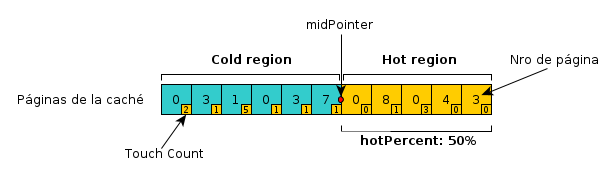
\includegraphics[scale=0.65]{diagramas/TouchCountAlgorithm1.png}\\
\end{center}

En la figura puede verse que Touch Count se cuenta con dos elementos, una lista y un puntero. La lista se utilizar\'a para manejar las p\'aginas y las prioridades que se le asignar\'an a cada
una esta lista estar\'a dividida en dos \'areas o regiones. La regi\'on de la izquierda de la lista denominada \textit{regi\'on fria} y la regi\'on inmediata
contigua denominada \textit{regi\'on caliente}.\\

Ambas regiones estar\'an separadas por un puntero, al que llamaremos midPointer, que se encargar\'a de marcar dicha divisi\'on. 
En realidad en la implementaci\'on el \textit{midpointer} estar\'a apuntando el primer elemento de la \textit{regi\'on caliente} cuando haya
elementos dicha regi\'on o a null en caso contrario.\\



Ahora describiremos su comportamiento en base a las operaciones que se realizan sobre la cach\'e.

\begin{itemize}
	\item{Agregar una p\'agina
		Si la cach\'e todav\'ia posee espacio disponible.
	}
	\item{Encontrar víctima }
	\item{Remover una p\'agina}
\end{itemize}



Peor caso del TouchCount

Si se referencian set de datos diferentes (tablas diferentes) cada vez, no se aclcanzaran para las paginas un aging count suficiente
para salvarlas y todo el tiempo estaremos pisando las página de la caché con páginas nuevas (al menos en la cola de frias)

Si nada se pasa del agingHot lo que esté en la Hot nunca se va a desaloar, sino que la cola cold será la que se renueve.
Se le va a dar más importancia a las páginas con touch counte mayor al aging count más nuevas.

\newpage
\section{Test de Unidad}

\newpage
\section{Comparaci\'on de Touch Count}

\subsection{Trazas}

\begin{itemize}
	\item{ Peor caso MRU: Traza MRUPathological
	}
		\begin{center}
		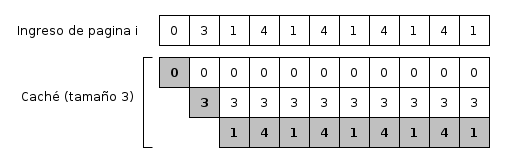
\includegraphics[scale=0.65]{diagramas/MRUPathological.png}\\
		\end{center}

	\item{ Peor caso LRU}
		\begin{center}
		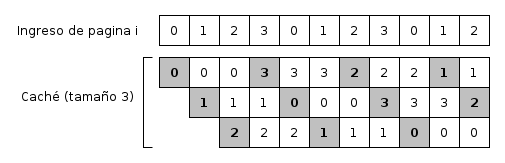
\includegraphics[scale=0.65]{diagramas/LRUPathological.png}\\
		\end{center}

	\item{ TouchCount vs LRU}
	\item{ Mejor caso LRU}
	\item{ Mejor caso MRU}
	\item{ Mejor caso \textit{Touch Count}}
	\item{ Peor caso \textit{Touch Count}}
\end{itemize}

\end{document}
